% §7 Self-decomposability and the characterization theorem --- blueprint chapter 7
% (blueprint/src/parts/07-characterization.tex), statements and proofs of record verbatim.
% Drafted 2026-09-11.
%
% Contents and departures from the blueprint chapter:
%   - all six statement nodes transcribed (lem:selfdecomposable-exponents,
%     thm:main-characterization, cor:semigroup-case, lem:admissible-cone,
%     prop:strict-positivity, prop:kernel-regularity) under their markers; five are [T] and
%     \leanok, and every proof is the machine-checked route as the
%     blueprint's CHANGED markers record; prop:kernel-regularity is [A] on A8 and A9, whose page
%     anchors are printed before it, with the F6-1 narrowing said in prose (the density may be
%     unbounded at the origin);
%   - the lead paragraphs are the blueprint's, with the draft's note on the letters; the reading
%     of the headline (what the axioms leave free) and its trust base are prose after the
%     theorem; the three remarks (rem:sato-process, rem:boundary, rem:scale-evolution-preview)
%     are copied, the last sentence of rem:boundary (the causal drift axiom) moved into this
%     section's one relation-to-the-causal-theory remark, rem:causal-relation-characterization,
%     which also carries the trust-base comparison (the analysis direction is proved here where
%     the causal article cites it) and the two facts that changed sides of the gauge argument;
%   - the blueprint's chapter references become section references.
% Forward references resolved for v0.1 (2026-09-12): lem:cin-rays is Appendix A; the pointers to
% chapters 10-12 are reworded as outside this paper; rem:gaussian-extreme (paper-only) is added
% after lem:admissible-cone for the extreme-ray claim of §§1 and 3.

\section{Self-decomposability and the characterization theorem}\label{sec:characterization}

This section turns the similarity form of \S\ref{sec:covariance} into a condition on one
function $F$, solves that condition, and states the classification
(Theorem~\ref{thm:main-characterization}). By Lemma~\ref{lem:additivity} the exponent of a
kernel is a difference of accumulated
exponents, and by Proposition~\ref{prop:canonical-gauge} the accumulated exponent is a dilate
of one function. So every kernel is read off $F$ by stretching its argument and subtracting,
\[
  g_{s,t}(\omega) = F(\tilde t\,\omega) - F(\tilde s\,\omega),
  \qquad \tilde s = \chi(s) \le \tilde t = \chi(t),
\]
and since $\chi$ is onto, $(\tilde s,\tilde t)$ ranges over all pairs $0 \le \tilde s \le
\tilde t$. Theorem~\ref{thm:increments-levy} requires each of these differences to be a
symmetric \Levy{} exponent. The pairs with $\tilde s = 0$ ask only that the dilates
$F(\tilde t\,\cdot)$ lie in $\LEs$, which they do. The content is in the pairs
$0 < \tilde s \le \tilde t$. That is a condition on $F$ alone, that every stretched
difference is a \Levy{} exponent, and it is the condition this section solves.

Canonical-gauge scales are written $s \le t$, plain, when no other family is in play,
so that $a$ is free for the Gaussian coefficient.

The condition is self-decomposability of the law of the displacement at unit scale. Let
$X_1$ be the random displacement whose law is the kernel at canonical scale $1$, so that
$\Ex\cos(\omega X_1) = e^{-F(\omega)}$. In the
canonical gauge the kernel at scale $t$ is the law of $tX_1$. That $F(\omega) - F(c\omega)$ is
a \Levy{} exponent for $c \in (0,1)$ says that there is a random variable $R_c$, independent of
$X_1$, with $X_1 \seq cX_1 + R_c$. That is self-decomposability
(Definition~\ref{def:self-decomposable}): covariance turns a shrinking of the scale axis into
a shrinking of the displacement, and the cascade requires what remains to be a measurement in
its own right. The lemma below is the analytic form of this statement, and
Figure~\ref{fig:profile} draws what it says about the profile. Its proof of (1) implies (3)
uses two facts about a nonincreasing profile that are stated in the appendix, because they
belong to the geometry of the cone: the tail measure $\varpi = -dk$ it attaches, and the
growth of $\Cin$ at infinity (Lemma~\ref{lem:cin-rays}).

% The displacement profile and its dilates: what the self-decomposability condition means.
% Paper-only figure (2026-09-14, the presentation review's one missing figure); the image is
% figures/fig-profile.png from scripts/make-fig-profile.py (numpy + matplotlib, no data).
\begin{figure}[t]
\centering

\includegraphics[width=\textwidth]{fig-profile.png}
\caption{The condition of Lemma~\ref{lem:selfdecomposable-exponents}, drawn for the profile
$k(x) = 2e^{-x}$ of the second member of \S\ref{sec:axioms}. Left: the profile at scales
$s = 1$ and $t = 2$ is the same function dilated, $k(x/s)$ and $k(x/t)$, and the increment
from $s$ to $t$ has profile $k(x/t) - k(x/s)$, the shaded difference. The difference is
nonnegative for every $s < t$ exactly when $k$ is nonincreasing, which is what makes the
increment a symmetric \Levy{} exponent. Right: in the log-displacement coordinate
$\theta = \log x$ the dilates are translates of one function $\tilde k(\theta) = k(e^\theta)$,
shifted by $\log(t/s)$, and the condition says that the profile can only rise as one moves
to finer scales.}
\label{fig:profile}
\end{figure}


% shared with blueprint lem:selfdecomposable-exponents
\begin{lemma}[symmetric self-decomposable exponents]\label{lem:selfdecomposable-exponents}
For $F \in \LEs$ with pair $(a,\nu)$ the following are equivalent.
\begin{enumerate}
\item $F(t\,\cdot) - F(s\,\cdot) \in \LEs$ for all $0 < s \le t$.
\item $F$ is continuously differentiable on $(0,\infty)$ and the symbol
$B(\omega) := \omega F'(\omega)$ lies in $\LEs$.
\item $F$ has the representation \ref{eq:sd-profile}: $\nu(dx) = k(x)\,x^{-1}dx$ with
$k : (0,\infty) \to [0,\infty)$ nonincreasing, $\int_0^1 x\,k(x)\,dx < \infty$ and
$\int_1^\infty k(x)\,x^{-1}dx < \infty$.
\end{enumerate}
In (3) the profile $k$ may be taken right-continuous with $k(\infty) = 0$, and then
$\varpi := -dk$ is a positive measure on $(0,\infty)$ with $k(x) = \varpi((x,\infty))$,
$\int (1 \wedge u^2)\,\varpi(du) < \infty$ and $\int \log_+ u\,\varpi(du) < \infty$; in (2) the
pair of $B$ is $(2a,\varpi)$.
\end{lemma}

The three conditions are not equally deep, and the asymmetry organizes what follows. (3)
implies (1) is elementary (a change of variables in the representation, using no property
of the positive definite class), and it is all the constructive direction of
Theorem~\ref{thm:main-characterization} uses. (1) implies (3) reads the dilation
identity backwards and then argues about monotone measures, elementary but genuine. It is
the analysis direction of the main theorem. (2) is here a consequence rather than a stepping
stone, because the line offers no a priori differentiability. What the superposition
\ref{eq:cin-superposition} buys instead is that
every admissible exponent is $C^1$ off the origin with a symbol that is again a \Levy{}
exponent. The whole lemma uses the uniqueness clause of
Proposition~\ref{prop:fourier-toolbox}(3) and nothing else, twice: once in (1) implies (3),
to read the dilation identity backwards, and once in (2) implies (3), to match the pair of
$F$ with the pair the profile produces. The lemma is the one-dimensional case of the
classical description of self-decomposable laws by their \Levy{} measures,
Proposition~\ref{prop:sd-exponents}, which is therefore cited for orientation and not used.
The tail measure $\varpi$ with its logarithmic moment is likewise classical: it is the
\Levy{} measure of the background driving \Levy{} process $Y$ of Jurek and Vervaat, whose
integral $\int_0^\infty e^{-s}\,dY(s)$ represents every self-decomposable law and converges
exactly when $\Ex\log(1 + |Y(1)|) < \infty$ (\sscite{jurek1983integral}, p.~247 and
Thm.~2.3, pp.~250--251).

\begin{proof}
\emph{(3) implies (1): the dilation identity.} Write
$F(c\omega) = ac^2\omega^2 + \int_0^\infty (1 - \cos c\omega x)\,k(x)\,\frac{dx}{x}$ for
$c > 0$ and substitute $u = cx$. The measure $dx/x$ is invariant under dilations, so
\[
  F(c\omega) = a c^2\,\omega^2
   + \int_0^\infty \bigl(1 - \cos\omega u\bigr)\,k(u/c)\,\frac{du}{u} :
\]
dilating the argument by $c$ dilates the profile and rescales the Gaussian coefficient, and
does nothing else. Subtracting the identity at $c = s$ from the one at $c = t$,
\begin{equation}\label{eq:dilation-difference}
  F(t\omega) - F(s\omega) = a(t^2 - s^2)\,\omega^2
   + \int_0^\infty \bigl(1 - \cos\omega u\bigr)\,\bigl(k(u/t) - k(u/s)\bigr)\,\frac{du}{u},
\end{equation}
which is of the form \ref{eq:levy-khintchine}: the Gaussian coefficient $a(t^2-s^2)$ is
nonnegative since $s \le t$, and the density is nonnegative since $u/t \le u/s$ and $k$ is
nonincreasing. For the \Levy{} condition, the density is dominated by $k(u/t)$, so it is enough
to bound the $(1 \wedge u^2)$-integral of $k(u/t)\,u^{-1}du$; and the same substitution
$u = tx$ turns that integral into $\int_0^\infty (1 \wedge t^2x^2)\,k(x)\,x^{-1}dx$, at most
$\max(1,t^2)\int_0^\infty (1 \wedge x^2)\,k(x)\,x^{-1}dx$, which is finite by
Lemma~\ref{lem:profile-integrability}; the comparison
$1 \wedge t^2x^2 \le \max(1,t^2)(1 \wedge x^2)$ holds in each of the two regimes of the
truncation separately. So the difference is itself of the form \ref{eq:levy-khintchine},
hence in $\LEs$; the class being named by its representation, this direction makes no appeal
to Proposition~\ref{prop:fourier-toolbox}.

\emph{(1) implies (3): the dilation identity read backwards, and the monotone density.} Fix
$c \in (0,1)$. By hypothesis $F(\omega) - F(c\omega) = a'\omega^2 + \int (1-\cos\omega
x)\,\nu'(dx)$ for some $a' \ge 0$ and some \Levy{} measure $\nu' \ge 0$. On the other hand, with
$\Dil{c}\nu$ the image of $\nu$ under $x \mapsto cx$, the first display of this proof reads
$F(c\omega) = ac^2\omega^2 + \int (1-\cos\omega x)\,(\Dil{c}\nu)(dx)$. Hence
\[
  a'\omega^2 + \int \bigl(1 - \cos\omega x\bigr)\,(\nu' + \Dil{c}\nu)(dx)
  \;=\; a\,\omega^2 + \int \bigl(1 - \cos\omega x\bigr)\,\nu(dx)
  \qquad \text{for every } \omega,
\]
an identity between two representations of the form \ref{eq:levy-khintchine} with
\emph{positive} data; so by the uniqueness clause of Proposition~\ref{prop:fourier-toolbox}(3),
$a' = a(1-c^2)$ and $\nu' + \Dil{c}\nu = \nu$. Thus
\begin{equation}\label{eq:dilation-decrease}
  \Dil{c}\nu \ \le\ \nu \qquad \text{for every } c \in (0,1).
\end{equation}
Pass to the log-displacement coordinate $\theta = \log x$: let $\tilde\nu$ be the image of
$\nu$ under $\log$, a measure on $\RR$ with
$\tilde\nu((\theta,\infty)) = \nu((e^\theta,\infty)) < \infty$ for every $\theta$, finiteness
coming from $\int (1 \wedge x^2)\,\nu < \infty$. Dilation by $c$ becomes translation by
$\log c < 0$, so \ref{eq:dilation-decrease} reads $\tilde\nu(A + h) \le \tilde\nu(A)$ for every
Borel $A$ and every $h > 0$: the measure decreases under every right shift. Put
\[
  \tilde k(\theta) \;:=\; \sup_{n \ge 0}\ 2^n\,\tilde\nu\bigl((\theta,\ \theta + 2^{-n}]\bigr).
\]
Each term is nonincreasing in $\theta$, by the shift property; and the sequence is nondecreasing
in $n$, because splitting $(\theta, \theta+2\delta]$ at its midpoint and applying the shift
property to the right half gives
$\tilde\nu((\theta,\theta+2\delta]) \le 2\,\tilde\nu((\theta,\theta+\delta])$. So $\tilde k$ is
nonincreasing, and it is a supremum of a nondecreasing sequence. Fix $a < b$. By monotone
convergence and then Tonelli,
\[
  \int_a^b \tilde k \;=\; \sup_n\ 2^n\!\int_a^b \tilde\nu\bigl((\theta,\theta+\varepsilon_n]\bigr)
    d\theta
  \;=\; \sup_n\ 2^n\!\int \bigl|(a,b] \cap [x - \varepsilon_n,\, x)\bigr|\ \tilde\nu(dx),
  \qquad \varepsilon_n = 2^{-n},
\]
and the inner length is $\varepsilon_n$ for $x \in (a+\varepsilon_n, b]$, at most
$\varepsilon_n$ always, and $0$ outside $(a, b+\varepsilon_n]$. So the $n$-th term lies between
$\tilde\nu((a+\varepsilon_n, b])$ and $\tilde\nu((a, b+\varepsilon_n])$, and both converge to
$\tilde\nu((a,b])$ --- the first by continuity of a measure from below, the second by continuity
from above, which is where the finiteness of the rays is used. Hence
$\tilde\nu((a,b]) = \int_a^b \tilde k$ for every $a < b$, so $\tilde\nu(d\theta) =
\tilde k(\theta)\,d\theta$. Returning to $x$, $\nu(dx) = k(x)\,x^{-1}dx$ with
$k(x) := \tilde k(\log x)$ nonincreasing; and $k(\infty) = 0$, since $\tilde k$ is nonincreasing
and nonnegative with $\int_\theta^\infty \tilde k = \tilde\nu((\theta,\infty)) < \infty$. The two
integrability conditions are $\int (1 \wedge x^2)\,\nu(dx) < \infty$ read through
Lemma~\ref{lem:profile-integrability}.

\emph{The measure $\varpi$, and the right-continuous profile.} A profile that is merely
nonincreasing has no right-continuous representative to hand, so the measure is built first and
the modification read off it. Take for $\varpi$ the measure Lemma~\ref{lem:cin-rays}(2)
attaches to $k$: the image of Lebesgue measure on $(0,\infty)$ under the generalized inverse
$y \mapsto \sup\{u > 0 : k(u) > y\}$, whose tails satisfy $\varpi((x,\infty)) = k(x)$ at every
continuity point of $k$, hence at almost every $x > 0$. Every positive tail is then finite,
since a point of that identity below $x$ bounds $\varpi((x,\infty))$ by a value of $k$; so
$k^{\ast}(x) := \varpi((x,\infty))$ is a finite nonincreasing function on $(0,\infty)$, equal to
$k$ almost everywhere and therefore inducing the same \Levy{} measure, right-continuous because
$(x,\infty)$ is the increasing union of the $(x + 1/n,\infty)$, and vanishing at infinity
because $k$ does. This is the modification the statement asserts, and its tail identity holds at
\emph{every} positive point rather than almost everywhere.

For the two integrability conditions, the layer cake formula against $\varpi$ turns
$\int G(u)\,\varpi(du)$, for $G(u) = \int_0^u g(t)\,dt$ with $g \ge 0$ continuous, into
$\int_0^\infty k^{\ast}(t)\,g(t)\,dt$. Take $g(t) = 2t(1+t^2)^{-2}$, so that
$G(u) = u^2/(1+u^2) \ge \tfrac12 (1 \wedge u^2)$, and note $g(t) \le 2t$ and
$g(t) \le 2t^{-1}$; then
$\int (1 \wedge u^2)\,\varpi(du) \le 4\int_0^1 t\,k(t)\,dt + 4\int_1^\infty k(t)\,t^{-1}dt$.
Take $g(t) = t(1+t^2)^{-1}$, so that $G(u) = \tfrac12\log(1+u^2) \ge \log_+ u$, with the same
two bounds on $g$; then $\int \log_+ u\,\varpi(du)$ is bounded by the same two integrals. So
both conditions on $\varpi$ follow from $\int_0^1 x\,k(x)\,dx < \infty$ and
$\int_1^\infty k(x)\,x^{-1}dx < \infty$.

\emph{(3) implies (2): the $\Cin$ superposition.} Tonelli over $\{0 < x < u\}$ turns
\ref{eq:sd-profile} into
\begin{equation}\label{eq:cin-superposition}
  F(\omega) = a\,\omega^2 + \int_{(0,\infty)} \Cin(\omega u)\,\varpi(du),
  \qquad \Cin(z) := \int_0^{z}\frac{1 - \cos v}{v}\,dv,
\end{equation}
since $\int_0^u (1-\cos\omega x)\,x^{-1}dx = \Cin(\omega u)$; the measure $\varpi$ is the one
supplied above, and only its almost-everywhere tail identity is used. The integrand
$v \mapsto (1-\cos v)/v$ of $\Cin$ is continuous at the origin as well, its value there being
$0$ and $|(1-\cos v)/v| \le |v|/2$; so $\Cin$ is continuously differentiable on all of $\RR$
with $\Cin'(v) = (1-\cos v)/v$, and
$\partial_\omega \Cin(\omega u) = u\,\Cin'(\omega u) = (1 - \cos\omega u)/\omega$. For $\omega$
in the interval $(\omega_0/2, 2\omega_0)$ this is bounded by
$(4\omega_0^{-1} + 2\omega_0)(1 \wedge u^2)$ --- it is at most $2/\omega$ and at most
$\omega u^2/2$, which are the two regimes of the truncation --- and $1 \wedge u^2$ is
$\varpi$-integrable, as the previous paragraph shows for every such $\varpi$. So
differentiation under the integral sign applies at every $\omega > 0$, and
\begin{equation}\label{eq:symbol}
  B(\omega) = \omega F'(\omega)
   = 2a\,\omega^2 + \int_{(0,\infty)} \bigl(1 - \cos\omega u\bigr)\,\varpi(du),
\end{equation}
which is of the form \ref{eq:levy-khintchine} with pair $(2a,\varpi)$, hence in $\LEs$ --- the
class being named by its representation, so exhibiting the pair is the conclusion and no appeal
to Proposition~\ref{prop:fourier-toolbox} is made. That $F$ is $C^1$ on $(0,\infty)$ and not
merely differentiable is a second dominated-convergence argument: $1 - \cos\omega v$ is
bounded by $(2 + (|\omega_0|+1)^2)(1 \wedge v^2)$ for $\omega$ within $1$ of $\omega_0$, so
$\omega \mapsto \int (1 - \cos\omega v)\,\varpi(dv)$ is continuous on $\RR$ and $F' $ is
continuous where $\omega \ne 0$. Both sides of \ref{eq:symbol} are stated at every real
$\omega$: the identity extends to $\omega < 0$ because $F$ is even, hence $F'$ odd, and holds
at $\omega = 0$ because the factor $\omega$ annihilates whatever value the derivative is
assigned there. (The half-line route, differentiating under the integral in the profile form
and applying Tonelli, is not available here: $\omega\sin(\omega x)$ is not of one sign, and
$\int u\,\varpi(du)$ may diverge, as it does for the stable profiles of index below $1$. The
$\Cin$ form has a positive integrand and needs no such integral. Nor is the profile form saved
by the two admissibility conditions: $k(x) = (\log x)^{-2}$ at infinity satisfies
$\int_1^\infty k(x)x^{-1}dx < \infty$ while $\int_1^\infty k(x)\,dx$ diverges, and that
integral is what dominating $|\sin(\omega x)|k(x)$ would need.)

\emph{(2) implies (3).} Let $B = \omega F'$ have pair $(a_B,\varpi)$ and put
$k(x) := \varpi((x,\infty))$, which is nonnegative and nonincreasing on $(0,\infty)$ and finite
at every positive $x$, since $\int (1 \wedge u^2)\,\varpi(du) < \infty$ bounds
$\varpi((x,\infty))$ by $(1 \wedge x^2)^{-1}$ times that integral. The claim is that $F$ is
\ref{eq:sd-profile} at the data $(\tfrac12 a_B, k)$, and the two integrability conditions on
$k$ come from two different places --- which is the order the proof has to be read in, because
the data is not admissible until both are in hand.

The first is the \Levy{} condition on $\varpi$ alone. The layer cake formula of the previous
paragraph, read from right to left at $g(t) = 2t(1+t^2)^{-2}$, turns
$\int_0^\infty k(t)\,g(t)\,dt$ into $\int u^2(1+u^2)^{-1}\,\varpi(du)$, at most
$\int (1 \wedge u^2)\,\varpi(du)$; and $g(t) \ge t/2$ on $(0,1)$, so
$\int_0^1 t\,k(t)\,dt \le 2\int (1 \wedge u^2)\,\varpi(du) < \infty$.

The second is not implied by the \Levy{} condition: $\varpi(du) = du/(u\log^2 u)$ on $(2,\infty)$
has finite truncated integral and divergent logarithmic one. What supplies it is the finiteness
of $F$. Since $B \ge 0$, $F' \ge 0$ on $(0,\infty)$, so the fundamental theorem of calculus on
$[\varepsilon,1]$ gives $\int_\varepsilon^1 F'(v)\,dv = F(1) - F(\varepsilon) \le F(1)$ for
every $\varepsilon \in (0,1)$, and letting $\varepsilon \downarrow 0$ along a sequence ---
monotonically, the integrand being nonnegative --- $\int_0^1 F'(v)\,dv \le F(1) < \infty$.
Now $F'(v) \ge v^{-1}\int (1 - \cos vu)\,\varpi(du)$, and Tonelli over
$(0,1) \times (0,\infty)$ with a positive integrand, together with the substitution
$\int_0^1 (1 - \cos uv)\,v^{-1}dv = \Cin(u)$, turns the integral of that lower bound into
$\int \Cin(u)\,\varpi(du)$. So $\int \Cin(u)\,\varpi(du) \le F(1) < \infty$. Since
$\Cin \ge 0$ everywhere and $\Cin(u) = \log u + O(1)$ at infinity
(Lemma~\ref{lem:cin-rays}(1)), $\log_+ u \le \Cin(u) + C\,(1 \wedge u^2)$ for a fixed $C$, so
$\int \log_+ u\,\varpi(du) < \infty$; the second layer cake, at $g(t) = t(1+t^2)^{-1}$, which
is at least $(2t)^{-1}$ beyond $1$, converts that into $\int_1^\infty k(t)\,t^{-1}dt < \infty$.

So $(\tfrac12 a_B, k)$ is admissible data, and defines an exponent $\tilde F$ of the form
\ref{eq:sd-profile}. It is $F$, and the identification does not re-derive the representation:
by \ref{eq:symbol} applied to $\tilde F$, whose profile has $\varpi$ for its tail measure,
$\omega\tilde F'(\omega) = a_B\omega^2 + \int (1 - \cos\omega u)\,\varpi(du) = B(\omega)
 = \omega F'(\omega)$ at every real $\omega$, so $\tilde F$ and $F$ have the same derivative at
every $\omega > 0$; both are continuous and vanish at the origin, so they agree on $[0,\infty)$
--- a function continuous on $[0,\infty)$ with vanishing derivative on $(0,\infty)$ is constant
on every $[\varepsilon, \omega]$, and its value at the origin is the limit of those constants
--- and both are even, so they agree on $\RR$. The uniqueness clause of
Proposition~\ref{prop:fourier-toolbox}(3), applied to the two representations of that one
function, then identifies the pairs: $a = \tfrac12 a_B$ and $\nu(dx) = k(x)\,x^{-1}dx$, which
is (3).
\end{proof}

% blueprint rem:sato-process, copied
\begin{remark}[the probabilistic reading]\label{rem:sato-process}
Together with the similarity structure, \ref{eq:sd-profile} says that the kernels are the
marginal laws of a \emph{symmetric self-similar additive process}: a process
$(X_{\tilde t})_{\tilde t \ge 0}$ on $\RR$ with independent, symmetric, not necessarily
stationary increments satisfying $X_{\lambda\tilde t} \seq \lambda X_{\tilde t}$, the Sato process of
exponent $1$ attached to the self-decomposable law of $X_1$. The paths oscillate, and the
Gaussian coefficient $a$ sets the variance $2a\tilde t^{\,2}$ of their continuous part. Nothing in the proofs uses this
correspondence, which is stated as a reading and grounds no statement.
\end{remark}

% shared with blueprint thm:main-characterization
\begin{theorem}[main theorem]\label{thm:main-characterization}
A family $(\Phis{s}{t})_{0 \le s \le t}$ satisfies (A1)--(A8) and (ND) \emph{if and only if}
there are an increasing bijection $\chi$ of $[0,\infty)$, the gauge, and a function $F$ of the
form \ref{eq:sd-profile} with $F \not\equiv 0$, such that
\[
  \Phis{s}{t} f = \mu_{s,t} * f, \qquad
  \hat\mu_{s,t}(\omega) = \exp\bigl[-\bigl(F(\chi(t)\,\omega) - F(\chi(s)\,\omega)\bigr)\bigr].
\]
In the canonical gauge the kernel at scale $t$ is the symmetric probability measure $\phi_t$
with $\hat\phi_t = e^{-F(t\,\cdot)}$, and the pair $(\chi,F)$ is unique up to the normalization
$\chi(1) = 1$.
\end{theorem}

Read against the axioms: the apertures are the marginal laws of one symmetric self-similar
additive process, the kernel at canonical scale $t$ being the law of $tX_1$, so the whole
family is generated by one law and the gauge. In the canonical gauge, what the axioms leave
free is exactly the pair $(a,k)$ of \ref{eq:sd-profile}: a Gaussian variance and a
nonincreasing displacement profile.
The Gaussian scale space is $(a,0)$. Everything else has a catalogue of jumps. The theorem is
machine-checked in all three clauses (construction, analysis, uniqueness) and its trust
base is Lean core together with two cited facts and no more: Bochner's theorem in the forward
direction, and the symmetric \Levy--Khintchine representation at its converse and its
uniqueness clauses (\S\ref{sec:machine-checked}). The kernels have densities as well,
unimodal about the origin, but that is Proposition~\ref{prop:kernel-regularity} and not this
theorem: the statement here is about measures, deliberately, absolute continuity resting on a
cited interface that the theorem does not use. A reader who wants the density should read the
two together.

\begin{proof}
\emph{Necessity.} Lemma~\ref{lem:convolution-representation}, Lemma~\ref{lem:nonvanishing},
Lemma~\ref{lem:additivity}, Theorem~\ref{thm:increments-levy},
Lemma~\ref{lem:covariance-fourier}, Lemma~\ref{lem:action-rigidity} and
Proposition~\ref{prop:canonical-gauge} together give the representation with
$F = G(1,\cdot) \in \LEs$ and $F \not\equiv 0$. Every increment
$F(\chi(t)\,\cdot) - F(\chi(s)\,\cdot) = g_{s,t}$ lies in $\LEs$ by
Theorem~\ref{thm:increments-levy}, and $\chi$ is onto $(0,\infty)$ by
Proposition~\ref{prop:canonical-gauge}, so condition (1) of
Lemma~\ref{lem:selfdecomposable-exponents} holds for every pair $0 < \tilde s \le \tilde t$ of
canonical scales, and that lemma yields \ref{eq:sd-profile}. The gauge so obtained is already
\emph{normalized}: it is the inverse of the orbit coordinate $c(\lambda) = S_\lambda 1$, which
fixes $1$ by Proposition~\ref{prop:canonical-gauge}, so $\chi(1) = 1$. What this direction
returns is therefore a normalized representation --- one of those the uniqueness clause
compares --- and not merely a representative of its orbit under
$(\chi,F) \mapsto (c\,\chi,\ F(c^{-1}\,\cdot))$.

\emph{Sufficiency.} Let $F$ be of the form \ref{eq:sd-profile} with $F \not\equiv 0$, and work
in the canonical gauge. For $0 \le s \le t$ the function
$g_{s,t}(\omega) := F(t\omega) - F(s\omega)$ lies in $\LEs$ by
Lemma~\ref{lem:selfdecomposable-exponents}, (3) implies (1) --- for $s = 0$ the increment is
$F(t\,\cdot)$ itself, which is in $\LEs$ by hypothesis and the dilation identity --- so by the
converse half of Proposition~\ref{prop:fourier-toolbox}(3) and by
Proposition~\ref{prop:fourier-toolbox}(1), $e^{-g_{s,t}}$ is the transform of a unique
probability measure $\mu_{s,t}$ on $\RR$, symmetric because the transform is real and even.
Put $\Phis{s}{t}f := \mu_{s,t} * f$. Then (A1)--(A5) hold by the converse direction of
Lemma~\ref{lem:convolution-representation}; (A6) because the exponents add and transforms
determine measures (Proposition~\ref{prop:fourier-uniqueness}); (A8) with
$S_\lambda t = \lambda t$, since $\hat\mu_{\lambda s,\lambda t}(\omega) =
\hat\mu_{s,t}(\lambda\omega)$; and (ND) because $F(t\,\cdot) - F(s\,\cdot) \not\equiv 0$ for
$s < t$: at $s = 0$ that is $F \not\equiv 0$, and for $s > 0$, if the increment vanished
identically then $F(\omega) = F(c\omega)$ for every $\omega$ with $c = s/t \in (0,1)$, whence
$F \equiv 0$ by Lemma~\ref{lem:dilation-invariance}. Only that \emph{some} frequency is moved
is needed here, which is less than Proposition~\ref{prop:strict-positivity}(2) asserts.

For (A7), a collapsing-increment estimate does the work. For a probability measure $\mu$ and
$f \in \Lone$ the $\Lone$ distance from $\mu * f$ to $f$ is at most $\int \Theta_f(y)\,\mu(dy)$,
where $\Theta_f(y)$ is the $\Lone$ distance from $\Tr{y}f$ to $f$; and $\Theta_f$ is bounded,
continuous, and vanishes at the origin, because the translation group acts continuously on
$\Lone$. So if $(s_n,t_n) \to (c,c)$ along admissible pairs then $\hat\mu_{s_n,t_n} \to 1$
pointwise, by continuity of $F$ and of $\chi$; hence $\mu_{s_n,t_n} \to \delta_0$ weakly by
Proposition~\ref{prop:levy-continuity}, hence
$\int \Theta_f(y)\,\mu_{s_n,t_n}(dy) \to 0$: a collapsing increment tends to the identity in
the strong operator topology. At a pair $s < t$ the two endpoints are then moved separately
--- there is no $t - s$ to move, this being a hemigroup: the left endpoint through an
increment applied \emph{first}, where the contraction property absorbs it, and the right
endpoint through one applied \emph{last}, where the same estimate is read at the image. No
compact set, no density argument and no $\varepsilon/3$ are needed.

Finally, for an arbitrary gauge $\chi$ set $\Phi'_{s,t} := \Phi_{\chi(s),\chi(t)}$: (A1)--(A6)
and (ND) hold verbatim, (A7) because an increasing bijection of $[0,\infty)$ is continuous ---
it is an order isomorphism of $[0,\infty)$ onto itself, and an order isomorphism between linear
orders carrying the order topology is a homeomorphism --- and (A8) with
$S'_\lambda = \chi^{-1}(\lambda\,\chi(\cdot))$.

\emph{Uniqueness.} The exponents $g_{0,t}$ are determined by the family: the kernels by
Lemma~\ref{lem:convolution-representation}, their transforms by
Proposition~\ref{prop:fourier-uniqueness}, and $-\log$ is single-valued on them by
Lemma~\ref{lem:nonvanishing}. The normalization $\chi(1) = 1$ recovers $F = g_{0,1}$; without
it the pair is determined up to $(\chi,F) \mapsto (c\,\chi,\ F(c^{-1}\,\cdot))$ with $c > 0$,
which is the freedom the normalization removes. For each $t$, $\chi(t)$ is then the unique
$c$ with $g_{0,t} = F(c\,\cdot)$: such a $c$ exists by the representation, and if
$F(c\omega) = F(c'\omega)$ for every $\omega$ with $c/c' \ne 1$, then $F \equiv 0$ by
Lemma~\ref{lem:dilation-invariance}, a contradiction.
\end{proof}

% shared with blueprint cor:semigroup-case
\begin{corollary}[recovering the semigroup case]\label{cor:semigroup-case}
Assume in addition that the family is one-parameter, that is, $\Phis{s}{t}$ depends only on
$t - s$. Then, after the normalization $g_{0,1}(1) = 1$,
\[
  F(\omega) = |\omega|^\alpha \quad \text{for some } 0 < \alpha \le 2 :
\]
the kernels are exactly the symmetric stable densities, which are the members of the extended
semigroup class of \sscite{pauwels1995extended} with positive kernels. Here $\alpha = 2$ is the
Gaussian, and $0 < \alpha < 2$ has Gaussian coefficient $0$ and profile
$k(x) = C_\alpha^{-1}x^{-\alpha}$ with
$C_\alpha := \int_0^\infty (1 - \cos u)\,u^{-1-\alpha}du \in (0,\infty)$.
\end{corollary}

The semigroup case is thus recovered from inside the hemigroup theory. The bound
$\alpha \le 2$ comes from Lemma~\ref{lem:quadratic-growth} rather than from a cited growth estimate.

\begin{proof}
\emph{The exponent is linear in the scale.} One-parametricity makes $\Phis{0}{t}$ and
$\Phis{s}{s+t}$ the same operator, so the uniqueness half of
Lemma~\ref{lem:convolution-representation} makes $\mu_{0,t}$ and $\mu_{s,s+t}$ the same
measure, and Lemma~\ref{lem:additivity} then reads $G(s+t,\omega) = G(s,\omega) + G(t,\omega)$
for all $s,t \ge 0$: the accumulated exponent is additive in the scale. It is continuous
there as well (Lemma~\ref{lem:additivity}), and an additive function continuous on
$[0,\infty)$ is linear on it --- extend it oddly to $\RR$, where it stays additive and
continuous, and a continuous additive map between real vector spaces is $\RR$-linear. So
$g_{0,t} = t\,g$ with $g := g_{0,1}$.

\emph{The exponent is multiplicative in the frequency.} \ref{eq:similarity} at $t = 1$, read
through the previous paragraph on the left-hand side, is
$S_\lambda(1)\,g(\omega) = g(\lambda\omega)$ for every $\lambda > 0$ and every $\omega$. At
$\omega = 1$ the normalization $g(1) = 1$ gives $S_\lambda(1) = g(\lambda)$, so
$g(\lambda\omega) = g(\lambda)\,g(\omega)$: the multiplicative function is $g$ itself, and no
separate homomorphism has to be identified.

\emph{Cauchy.} $g$ is continuous (Lemma~\ref{lem:nonvanishing}) and strictly positive off the
origin (Lemma~\ref{lem:no-lattice}), so $u \mapsto \log g(e^u)$ is additive and continuous on
$\RR$, hence linear by the same theorem as above, and $g(\omega) = \omega^\alpha$ for
$\omega > 0$ with $\alpha := \log g(e)$. Evenness of the exponent extends the formula to
$\omega < 0$, and $g(0) = 0$ covers the origin once $\alpha \ne 0$ is known.

\emph{The index.} $\alpha > 0$ because $g$ is continuous at $0$ with $g(0) = 0$, while
$\omega^\alpha \ge 1$ on $(0,1]$ when $\alpha \le 0$. For the upper bound,
Lemma~\ref{lem:quadratic-growth} applied to the \Levy{} pair of $g$, which
Theorem~\ref{thm:increments-levy} supplies, gives a constant $C$ with
$g(\omega) \le C(1+\omega^2)$; the normalization $g(1) = 1$ forces $C \ge 1/2$, and if
$\alpha > 2$ then at $\omega := (2C+1)^{1/(\alpha-2)} \ge 1$ the left side is
$(2C+1)\,\omega^2 > C(1+\omega^2)$, which the bound forbids. So $\alpha \le 2$.

\emph{The profile.} When $0 < \alpha < 2$ the integral $C_\alpha$ converges, by the two regimes
of the truncation: $1 - \cos u \le u^2/2$ makes its integrand at most $u^{1-\alpha}/2$ near the
origin, integrable exactly for $\alpha < 2$, and $1 - \cos u \le 2$ makes it at most
$2u^{-1-\alpha}$ beyond $1$, integrable exactly for $\alpha > 0$. Those two comparisons
\emph{are} the two integrability conditions of \ref{eq:sd-profile} for
$k(x) = C_\alpha^{-1}x^{-\alpha}$, which is nonincreasing, with $a = 0$, so no separate appeal
is needed; and $C_\alpha > 0$ because its integrand is nonnegative and does not vanish on
$(0,1)$. The substitution $u = |\omega|x$, performed on the $[0,\infty]$-valued integral so that
integrability does not have to be revisited at each frequency, gives
$\int_0^\infty (1-\cos\omega x)\,x^{-1-\alpha}dx = C_\alpha|\omega|^\alpha$, hence the exponent
$|\omega|^\alpha$. When $\alpha = 2$, $k \equiv 0$ and $a = 1$.
\end{proof}

% blueprint rem:boundary, copied; its last sentence (the causal drift axiom) moved to
% rem:causal-relation-characterization below
\begin{remark}[the boundary, the Gaussian ray, and what is not there]\label{rem:boundary}
The boundary $\alpha = 2$ of the semigroup slice is the Gaussian, nothing is degenerate, and
the trace of the boundary in the general class is the Gaussian coefficient $a$, which adds
an independent Gaussian displacement of variance $2at^2$ to the kernel at scale $t$ and of
variance $2a(t^2 - s^2)$ to every increment. The members of
\sscite{pauwels1995extended}
beyond $\alpha = 2$ have positive transfer functions and sign-changing kernels. They are
excluded by (A4) through Theorem~\ref{thm:main-characterization}, and by nothing in
\S\S\ref{sec:representation} to~\ref{sec:covariance}. So positivity, rather than
recursivity, narrows the class.
\end{remark}

The admissible pairs $(a,k)$ are closed under sums and nonnegative multiples, so the
exponents, with the zero exponent adjoined, form a convex cone. What is read off it below is the position of the Gaussian ray and the
places of the named members (Figure~\ref{fig:admissible-cone}).

% shared with blueprint lem:admissible-cone
\begin{lemma}[the admissible exponents form a convex cone]\label{lem:admissible-cone}
If $F_1, F_2$ are admissible in the sense of Theorem~\ref{thm:main-characterization}, of the
form \ref{eq:sd-profile} with Gaussian coefficients $a_1, a_2 \ge 0$ and nonincreasing profiles
$k_1, k_2$, then so are $F_1 + F_2$, with data $(a_1+a_2, k_1+k_2)$, and $c\,F_1$ for $c \ge 0$,
with data $(c\,a_1, c\,k_1)$. So the admissible exponents form a convex cone, and the
correspondence with the pairs $(a,k)$ is linear.
\end{lemma}

\begin{proof}
Each defining condition --- nonnegativity of $a$, nonnegativity and monotonicity of $k$, and
the two integrability conditions --- is stable under sums and under multiplication by $c \ge 0$,
the last two because the integrands $x k(x)$ and $k(x)/x$ are nonnegative on $(0,\infty)$, so that
the integral of a sum is the sum of the integrals with no side condition. The same additivity,
applied to \ref{eq:sd-profile} at a fixed $\omega$, gives $F_1 + F_2$ and $c\,F_1$ as the
exponents of the summed and scaled data, as identities in $[0,\infty]$; they are identities
between real numbers because Lemma~\ref{lem:profile-integrability} makes each $F_i$ the
exponent of a symmetric \Levy{} pair and Lemma~\ref{lem:quadratic-growth} makes that finite at
every frequency.
\end{proof}

% paper-only observation (2026-09-12): the extreme-ray property of the Gaussian, which the
% blueprint proves in chapter 8 (prop:choquet-cone) together with the other extreme rays; here it
% is the one-line consequence of the linear correspondence with pairs that §§1 and 3 cite.
\begin{remark}[the Gaussian ray is extreme]\label{rem:gaussian-extreme}
The correspondence of Lemma~\ref{lem:admissible-cone} makes the Gaussian ray
$\{(a,0) : a \ge 0\}$ an extreme ray of the cone: if $(1,0) = (a_1,k_1) + (a_2,k_2)$ with both
summands admissible, then $k_1 + k_2 = 0$ with $k_1, k_2 \ge 0$ forces $k_1 = k_2 = 0$, so
both summands lie on the ray. Every admissible exponent is a superposition of the Gaussian
ray and the exponents of the unit-step profiles of Lemma~\ref{lem:cin-rays}
(\ref{eq:cone-superposition}). That does not by itself make the unit-step exponents extreme:
a family of rays can represent every point of a cone without each of its members being
indecomposable, as the points of a square's boundary represent every point of the square.
That the unit-step exponents are extreme, and that no other rays are, is outside this
paper. Figure~\ref{fig:admissible-cone} draws the cone with the members this paper names.
\end{remark}

% Figure: the admissible cone. Referenced from §7 after rem:gaussian-extreme. Pure TikZ, on the
% design of Paper I's fig-admissible-cone, redrawn for this article's cone and for what THIS
% paper shows: the Gaussian ray as an extreme ray (rem:gaussian-extreme), the Cin rays on the
% far boundary (Appendix A exhibits them; that they are the other extreme rays is outside the
% paper and the caption says so), the stable exponents as the semigroup slice
% (cor:semigroup-case), the Matern ray (Appendix A). No Thorin region, no collar.

\begin{figure}[t]
\centering
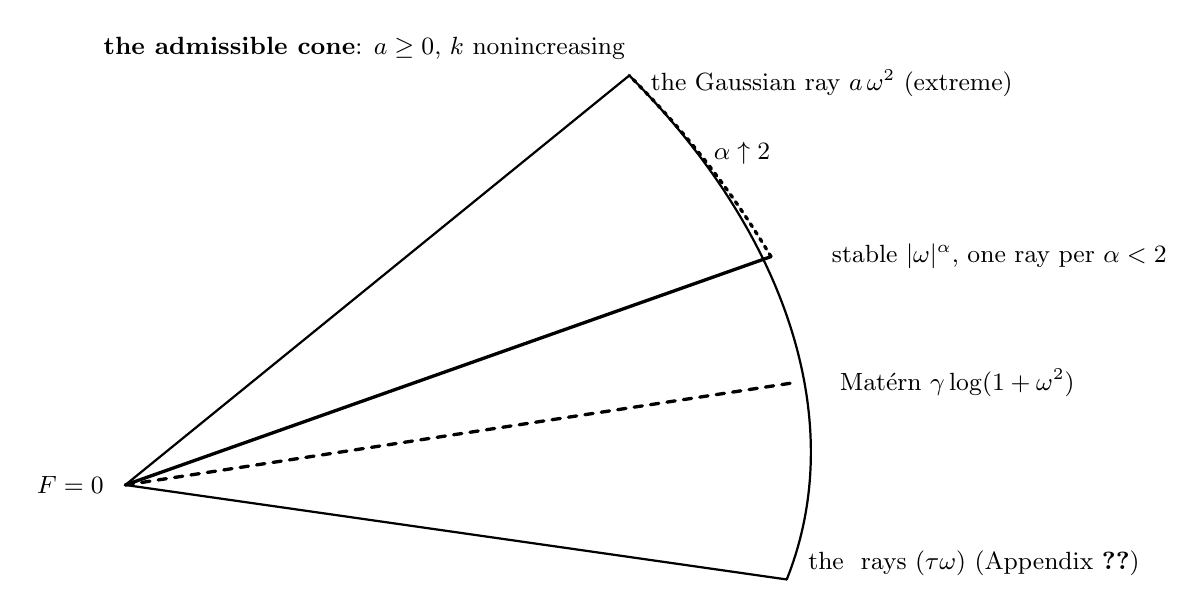
\begin{tikzpicture}[every node/.style={font=\small}, line cap=round, >=stealth]

% the cone, a wedge from the apex F = 0
\coordinate (O) at (0,0);
\draw[thick] (O) -- (6.4,5.2);     % upper edge: the Gaussian ray a omega^2
\draw[thick] (O) -- (8.4,-1.2);    % lower edge: a Cin ray
\draw[thick] (6.4,5.2) .. controls (8.4,3.2) and (9.2,0.8) .. (8.4,-1.2); % the far boundary: the Cin rays
\node[anchor=west] at (6.55,5.1) {the Gaussian ray $a\,\omega^2$ (extreme)};
\node[anchor=west] at (8.55,-1.0) {the $\Cin$ rays $\Cin(\tau\omega)$ (Appendix~\ref{sec:appendix})};
\node[anchor=east] at (-0.15,0) {$F = 0$};
\node[anchor=west] at (-0.4,5.55) {\textbf{the admissible cone}: $a \ge 0$, $k$ nonincreasing};

% the semigroup slice: the stable exponents, a curve of rays from alpha -> 0 to alpha = 2
\draw[very thick] (O) -- (8.2,2.9);
\node[anchor=west] at (8.85,2.9) {stable $|\omega|^{\alpha}$, one ray per $\alpha < 2$};
\draw[very thick,dotted] (8.2,2.9) .. controls (7.6,3.9) and (7.0,4.6) .. (6.4,5.2);
\node[anchor=south west] at (7.35,3.95) {$\alpha \uparrow 2$};
% the Matern ray
\draw[very thick,dashed] (O) -- (8.5,1.3);
\node[anchor=west] at (8.95,1.3) {Mat\'ern $\gamma\log(1+\omega^2)$};

\end{tikzpicture}
\caption{The admissible cone. Theorem~\ref{thm:main-characterization} identifies the
exponents $F$ with pairs $(a,k)$, a Gaussian coefficient and a nonincreasing profile, and
these form a convex cone (Lemma~\ref{lem:admissible-cone}). The Gaussian ray is an extreme
ray (Remark~\ref{rem:gaussian-extreme}), and it is a smoothing member, not a
degenerate boundary. The exponents of the unit-step profiles, the $\Cin$ rays of
Appendix~\ref{sec:appendix}, are the rays that generate the cone together with the Gaussian
ray: every admissible exponent is a superposition of them
(\ref{eq:cone-superposition}). They are drawn along the far side only to keep them apart;
whether they are extreme, which the superposition alone does not show, is outside this
paper, and the drawing places nothing. The semigroup case cuts the
slice of stable exponents $|\omega|^\alpha$ (Corollary~\ref{cor:semigroup-case}), one ray
for each $\alpha \in (0,2)$, and the slice ends on the Gaussian ray at $\alpha = 2$. The
Mat\'ern member of \S\ref{sec:axioms} is one ray, with the profile $2\gamma e^{-x}$
(Proposition~\ref{prop:matern-exponent}). The drawing is schematic: the cone is
infinite-dimensional.}
\label{fig:admissible-cone}
\end{figure}


Two facts that the earlier sections could not supply are here consequences of the
classification.

% shared with blueprint prop:strict-positivity
\begin{proposition}[strict positivity and monotonicity of the admissible exponents]
\label{prop:strict-positivity}
Let $F$ be of the form \ref{eq:sd-profile} with $F \not\equiv 0$.
\begin{enumerate}
\item $F$ is nondecreasing on $[0,\infty)$.
\item $F(t\omega) - F(s\omega) > 0$ for all $0 \le s < t$ and every $\omega \ne 0$.
Consequently, in the canonical gauge, no increment $\mu_{s,t}$ with $s < t$ is a lattice law,
and $G(\cdot,\omega)$ is strictly increasing for every $\omega \ne 0$.
\end{enumerate}
\end{proposition}

Clause (2) is what Corollary~\ref{cor:monotonicity} could not give before covariance and
Lemma~\ref{lem:no-lattice} gave only for the kernels from the origin: after the
classification the exceptional set is empty. So strict monotonicity in scale, and
monotonicity in the transform variable, both hold here: for the exponents the axioms
select, not for the class $\NDs$, in which Lemma~\ref{lem:lattice-zero} shows they are false.

\begin{proof}
(1) For $0 \le \omega_1 \le \omega_2$ the difference $F(\omega_2) - F(\omega_1)$ is the value at
frequency $1$ of the increment $F(\omega_2\,\cdot) - F(\omega_1\,\cdot)$, which lies in $\LEs$
by Lemma~\ref{lem:selfdecomposable-exponents}, (3) implies (1) --- at $\omega_1 = 0$ read as
the dilate $F(\omega_2\,\cdot)$ itself --- and a member of $\LEs$ is nonnegative. So
monotonicity is the dilation identity evaluated at one frequency, and no second change of
variables is needed.

(2) By the same formula, for $\omega > 0$ --- which suffices, $F$ being even ---
\[
  F(t\omega) - F(s\omega)
  = a(t^2-s^2)\omega^2
   + \int_0^\infty (1-\cos u)\,\bigl[k(u/(t\omega)) - k(u/(s\omega))\bigr]\,\frac{du}{u},
\]
with a nonnegative integrand, reading $k(u/(s\omega)) = k(\infty) = 0$ when $s = 0$. Suppose it
vanishes. Then $a = 0$, because $t^2 > s^2$ and $\omega \ne 0$; and the integral vanishes, so
its integrand vanishes for almost every $u > 0$, and since $1 - \cos u$ is positive off the
countable set $2\pi\ZZ$, which is null, $k(u/(t\omega)) = k(u/(s\omega))$ for almost every
$u > 0$. For $s = 0$ this says $k = 0$ almost everywhere, and $F \equiv 0$.

For $s > 0$ it says $k(\varkappa x) = k(x)$ for almost every $x > 0$, with
$\varkappa := t/s > 1$, and the tail integral finishes it. For every $\varepsilon > 0$ the
integral $J(\varepsilon) := \int_\varepsilon^\infty k(u)\,du/u$ is finite: bound $k(u)/u$ by
$k(\varepsilon)/\varepsilon$ on $(\varepsilon,1]$, using that $k$ is nonincreasing, and use
$\int_1^\infty k(u)\,u^{-1}du < \infty$ beyond $1$. The change of variables $u = \varkappa x$
carries $J(\varkappa\varepsilon)$ to $\int_\varepsilon^\infty k(\varkappa x)\,dx/x$, which is
$J(\varepsilon)$ by the almost-everywhere relation --- the measure $dx/x$ being invariant under
the multiplicative group. Splitting $J(\varepsilon)$ at $\varkappa\varepsilon$ and cancelling
the finite tail gives $\int_\varepsilon^{\varkappa\varepsilon} k(u)\,du/u = 0$; on that interval
$k$ is bounded below by $k(\varkappa\varepsilon)$, which must therefore vanish; and since
$\varepsilon$ was arbitrary, reading the conclusion at $\varepsilon = x/\varkappa$ gives
$k(x) = 0$ for every $x > 0$. So $F \equiv 0$ here too, which is excluded. No covering argument
and no passage from almost everywhere to everywhere is needed.

In the canonical gauge $g_{s,t} = F(t\,\cdot) - F(s\,\cdot)$, so $G(\cdot,\omega)$ is strictly
increasing for every $\omega \ne 0$; and if some increment $\mu_{s,t}$ were carried by a lattice
$p\ZZ$ then its cosine transform at $2\pi/p$ would be the integral of the constant $1$, hence
$1$, so $g_{s,t}(2\pi/p) = 0$ at a nonzero frequency, which the clause just proved forbids.
\end{proof}

The regularity of the kernels is classical and is cited rather than reproven. A
self-decomposable law on $\RR$ that is not a point mass is absolutely continuous
(\sscite{sato1999levy}, Thm.~27.13, p.~181, stated on $\RR^d$ and used for $d = 1$). A law
of class $L$ (the classical name for the self-decomposable laws,
Definition~\ref{def:self-decomposable}) is unimodal (\sscite{yamazato1978unimodality},
Thm.~1, p.~523), unimodality
meaning there that the distribution function is convex to the left of the mode and concave to
the right of it.

% shared with blueprint prop:kernel-regularity
\begin{proposition}[regularity of the kernels from the origin]\label{prop:kernel-regularity}
Let $(\Phis{s}{t})$ satisfy (A1)--(A8) and (ND). Then for every $t > 0$ the kernel $\mu_{0,t}$
is absolutely continuous, and its density is unimodal with mode at the origin.
\end{proposition}

\begin{proof}
For a nondegenerate self-decomposable law on $\RR$ the statement is the two cited facts:
absolute continuity is \sscite{sato1999levy}, Thm.~27.13, and unimodality is
\sscite{yamazato1978unimodality}, Thm.~1. What remains is the hypothesis check. That
$\mu_{0,t}$ is self-decomposable is Proposition~\ref{prop:canonical-gauge} with
Lemma~\ref{lem:additivity}: the factor law Definition~\ref{def:self-decomposable} asks for at
ratio $b$ is the increment $\mu_{t',t}$ at the scale $t'$ with $\chi(t') = \chi(t)/b$, which
exists because the gauge is onto $[0,\infty)$. That it is nondegenerate is the last clause
of Proposition~\ref{prop:canonical-gauge}, that some frequency is moved. The mode is at the
origin because the density is even: the set of modes of a unimodal law is an interval, and
for an even density that interval is symmetric about $0$, so it contains $0$.
\end{proof}

Two things the proposition does not say. It is made for the kernels \emph{from the origin} only: the
increments $\mu_{s,t}$ with $s > 0$ are infinitely divisible but not in general
self-decomposable, and nothing is claimed about them. And ``unimodal with mode at the
origin'' is a claim about the shape of the density, nonincreasing on $(0,\infty)$ and even,
and not about its value there, where the density need not be bounded.

That an exponent vanishing at one nonzero frequency vanishes identically is false for
$\NDs$ (Lemma~\ref{lem:lattice-zero}) but true, monotonicity in $\omega$ included, for the
exponents the axioms select (Proposition~\ref{prop:strict-positivity}). The axioms never
produce a multimodal kernel from the origin. No truncation of the Gaussian is admissible,
for a different reason: the transform of an even density carried by $[-R,R]$ with
$p(R-) > 0$ has the leading term $2p(R-)\sin(R\omega)/\omega$ as $\omega \to \infty$, by
integration by parts, so it changes sign, which Lemma~\ref{lem:nonvanishing} forbids; or,
more generally, an infinitely divisible law that is not a point mass has unbounded support
(\sscite{sato1999levy}, Cor.~24.4, p.~149).

% blueprint rem:scale-evolution-preview, copied; chapter references made section references
\begin{remark}[the scale evolution, in one line]\label{rem:scale-evolution-preview}
In the canonical gauge $\hat\phi_t(\omega) = e^{-F(t\omega)}$, so on the Fourier side the
family solves $\partial_t\hat u = -t^{-1}B(t\omega)\,\hat u$ with $B = \omega F'$ the symbol of
Lemma~\ref{lem:selfdecomposable-exponents}(2). By \ref{eq:symbol} that symbol is the
generator of the symmetric \Levy{} process with Gaussian part $2a$ and jump measure $\varpi$.
For the Gaussian, $B(\omega) = 2a\omega^2$ and the equation is the heat equation in the
variance gauge; for the Mat\'ern member, $F = \gamma\log(1+\omega^2)$ and
$B(\omega) = 2\gamma\omega^2/(1+\omega^2)$, a \emph{bounded} symbol. That the symbol be a
polynomial, so that the evolution is a differential equation in $x$, forces $\varpi = 0$ by
\ref{eq:symbol}. The equation and the observation are stated here without proof; the
evolution in generator form and the locality theorem they lead to are outside this paper.
\end{remark}

\begin{remark}[relation to the causal theory]\label{rem:causal-relation-characterization}
The characterization is the twin of the causal article's \sscite{fagerstrom2026hemigroup},
Laplace replaced by Fourier and the drift slot by the Gaussian slot, and three things differ
in how it is reached. The analysis direction of
Lemma~\ref{lem:selfdecomposable-exponents} is proved here, from the dilation identity and the
monotone density on the log-displacement axis, where the causal development cites the
classical characterization of self-decomposable \Levy{} measures and carries it in its trust
base. At this point the trust base of the present article is the narrower of the two. The two
facts of Proposition~\ref{prop:strict-positivity}, strict positivity of every increment off
the origin and monotonicity of $F$ in the transform variable, were available on the half-line
before the gauge argument, from the vanishing lemma and the monotonicity of Bernstein
functions, and are here consequences of the classification. This is the last of the three
substitutions announced in Remark~\ref{rem:causal-relation-covariance}. And the continuity
axiom in the sufficiency half is verified by a collapsing-increment estimate in place of the
$\varepsilon/3$ argument on a compact set, the machine-checked route in both articles. One
axiom does not transfer: the additional axiom that removed the drift in the causal theory has
a counterpart here, $\lim_{\omega \to \infty} F(\omega)/\omega^2 = 0$, which says $a = 0$.
Unlike its causal twin it would exclude the Gaussian, and this article
does not impose it.
\end{remark}
